\chapter{Noções preliminares}\label{Notions}


\begin{flushright}
\begin{minipage}[t][0cm][b]{0.47\textwidth}
\emph{Se você conhece o inimigo e conhece a si mesmo, não precisa temer o resultado de cem batalhas. }
\end{minipage}

\rule[0cm]{7cm}{0.03cm}%{largura}{espessura}

Sun Tzu
\end{flushright}

\section{Conceitos e definições iniciais}

Neste capítulo apresentaremos alguns conceitos que facilitarão o entendimento do problema estudado. Em geral, a maioria das notações utilizadas é simples, então vamos procurar ilustrar com exemplos somente aqueles conceitos e definições que fogem ao escopo básico da teoria de grafos. Como bibliografia básica sobre grafos sugerimos a leitura de~\cite{jayme2018}.

É importante ressaltar que em todo esse estudo, somente consideraremos grafos finitos, conexos e simples, ou seja, grafos sem
laços (aresta ligando um vértice nele mesmo) ou mais de uma aresta ligando dois
vértices.

A seguir descreve-se a terminologia e notação utilizada neste trabalho.

Um grafo $G$ é uma estrutura composta por dois subconjuntos finitos: $V(G)$ é o subconjunto cujos elementos são denominados \emph{vértices}, e $E(G)$ é subconjunto de pares não ordenados de elementos tomados de $V(G)$, os quais são chamados de \emph{arestas}. Uma aresta $e = (u,v)\in E(G)$ é formada pelo par de vértices $u,v \in V(G)$, neste caso $u$ e $v$ são ditos ser vértices \emph{adjacentes}. Dizemos também que  $e$ é \emph{aresta incidente} a $u$ e $v$. Denotamos a \emph{cardinalidade} de $|V(G)| = n$ e $|E(G)| = m$.

A \emph{vizinhança aberta} de um vértice $v\in V(G)$ é denotada $N(v) = \{u\in V(G) | (u,v) \in E(G)\}$. Já a \emph{vizinhança fechada} de um vértice $v\in V(G)$ é denotada $N[v] = N(v) \cup \{v\}$. 

Sejam $u, v$ vértices de $G$, se $N(u) = N(v)$ então $u$ e $v$ são ditos \emph{gêmeos falsos}, por outro lado, se $N[u] = N[v]$, então $u$ e $v$ são ditos \emph{gêmeos verdadeiros}. O \emph{grau de um vértice} $v$, denotado por $d(v)$, corresponde ao número de vértices adjacentes a $v$, ou seja, a cardinalidade de $|N(v)|$. O \emph{grau máximo} de um grafo $G$ é denotado por $\Delta(G) = max\{d(v) | v \in V(G)\}$. De forma similar o \emph{grau mínimo} é denotado por $\delta(G) = min\{d(v) | v \in V(G)\}$.

Dado um grafo $G$, e um vértice $v \in V(G)$, o grafo $G\backslash \{v\}$ é obtido a partir de $G$ retirando-se o vértice $v$ de seu conjunto de vértices, e retirando-se também todas arestas de $E(G)$ incidentes a $v$. De forma semelhante, dada uma aresta $e \in E(G)$, o grafo $G\backslash \{e\}$ é obtido a partir de $G$ retirando-se a aresta $e$ de $E(G)$.

Dizemos que $G'(V',E')$ é um \emph{subgrafo} de um grafo $G(V,E)$ quando $V'\subseteq V$ e $E'\subseteq E$. Quando o subgrafo $G'$ contém todas as arestas de $E$ cujas extremidades estão contidas em $V'$, então $G'$ é o \emph{subgrafo induzido} de $G$ por $V'$.  

Um grafo $G$ é um \emph{ciclo}, que denotaremos por $C_n$, se ele é uma sequência de vértices   $v_1, \dots, v_n, v_1$ distintos, onde $v_i \neq v_j$ para $i\neq j$ e $(v_i, v_{i+1})\in E(G)$,  tal que $n\geq 3$. 

Um grafo que não possui ciclos é dito \emph{acíclico}. Um grafo $G$ é \emph{conexo} se existe um caminho entre qualquer par de vértices de $G$. Um grafo é uma \emph{árvore} quando é acíclico e conexo. Um subgrafo conexo de uma árvore é dito \emph{subárvore}.

Um conjunto $\mathcal{S}$ é \emph{maximal} em relação a uma determinada propriedade $P$ se $\mathcal{S}$ satisfaz $P$, e todo conjunto $S'$ que contém propriamente $\mathcal{S}$ não satisfaz $P$. Analogamente, um conjunto $\mathcal{S}$ é \emph{minimal} em relação a uma determinada propriedade $P$ se $\mathcal{S}$ satisfaz $P$, e todo conjunto $S'$ que está contido propriamente em $\mathcal{S}$ não satisfaz $P$.

Um grafo $G$ é um \emph{grafo de intersecção} de uma família de subconjuntos de um conjunto $\mathcal{S}$, quando for possível associar cada vértice $v \in V(G)$ a um subconjunto $S_v \subseteq \mathcal{S}$, tal que $S_u \cap S_v \neq \emptyset$ se e somente se $(u,v)\in E(G)$. 


O termo \emph{grade} é utilizado para denotar o espaço Euclidiano de coordenadas ortogonais inteiras. Cada par de \emph{coordenadas} inteiras corresponde a um ponto ou vértice da grade. O termo \emph{aresta da grade}, será usado para denotar um par de vértices que estão a distância um na grade. Duas arestas $e_1$ e $e_2$ são \emph{arestas consecutivas} quando elas compartilham exatamente um ponto da grade.
 Um \emph{caminho na grade} é qualquer sequência finita de arestas consecutivas $e_1 = (v_1, v_{2}), e_2 = (v_2, v_{3}), \dots, e_i = (v_i, v_{i+1}), \dots, e_m = (v_{m}, v_{m+1})$,  onde   $v_i \neq v_j$ para $i \neq j$. A primeira e a última arestas de um caminho são chamadas \emph{arestas de extremidade}.
A \emph{direção de uma aresta} é vertical quando a primeira coordenada de seus vértices é igual, e é horizontal quando a segunda coordenada é igual. Uma \emph {dobra} em um caminho é um par de arestas consecutivas $ e_1, e_2 $ do caminho, tal que as direções de $ e_1$ e $ e_2$ são diferentes. Quando duas arestas $ e_1$ e $e_2 $ formam uma dobra, elas são chamadas \emph {arestas de dobra}. Um \emph {segmento} é um conjunto de arestas consecutivas de um caminho, sem repetição e sem dobra. %is a path with no bends.
 Dois caminhos são ditos   \emph{aresta-intersectantes}, ou simplesmente  \emph{intersectantes}, se eles compartilham pelo menos uma aresta. %Otherwise we say they are \emph{edge-disjoint} (or disjoint).
 No decorrer deste trabalho, a qualquer momento em que for citado que dois caminhos são intersectantes, em uma representação EPG, o que isso quer dizer é que eles são aresta-intersectantes. 
 
Grafos EPG são uma classe de grafos de intersecção de caminhos em grade~\cite{golumbic2009}. Essa classe consiste dos de grafos cujos vértices podem ser representados por caminhos de uma grade $ Q $, tal que dois vértices de  $ G $ são adjacentes se e somente se os caminhos correspondentes se intersectam. Se todo caminho em uma representação pode ser representado com no máximo $ k $ dobras, dizemos que esse grafo $ G $ possui uma representação \emph{$ B_k$-EPG}. Quando $ k = 1 $ dizemos que essa é uma representação de \emph{dobra simples}.


Dizemos que uma família $\mathcal{F}$ de conjuntos  é \emph{$k$-intersectante} se para todos $F_1, F_2, \dots, F_k$ subconjuntos de $\mathcal{F}$, temos que $F_1\cap F_2 \cap \dots \cap F_k \neq \emptyset$. Dizemos ainda que uma família $\mathcal{F}$  de conjuntos é \emph{$k$-Helly}, quando toda subfamília  $k$-intersectante $F'$ de $\mathcal{F}$ possui no mínimo um elemento comum.
Em específico, dizemos que uma família de conjuntos é  \emph{mutuamente intersectante}, i.e. dois a dois intersectante, se quaisquer dois conjuntos na família se intersectam. Uma coleção de conjuntos não vazios $C$ satisfaz a propriedade Helly, i.e. é $2$-Helly, quando toda subcoleção mutuamente intersectante $S$ de $ C $ possui no mínimo um elemento que está em todo subconjunto de $S$.

Por simplicidade, todas as vezes que nos referirmos a uma família de conjuntos dizendo que ela é uma família Helly está subentendido que na verdade essa família é $2$-Helly. %A omissão da impressão do número 2 em famílias $2$-Helly é comum, dessa forma, uma representação EPG-2-Helly é denotada simplesmente por EPG-Helly.

%Na álgebra booleana, uma \emph{conjunção} é uma operação lógica relacionada à intersecção de conjuntos que possui semântica de \textbf{and}. Uma \emph{disjunção} é uma operação lógica relacionada à intersecção de conjuntos que possui semântica de \textbf{or}. Um \emph{literal} é um átomo ou a negação de um átomo. Um \emph{átomo} é um literal positivo. A negação de um átomo é um literal negativo. 
Uma \emph{cláusula} é uma disjunção ou conjunção de literais. Dizemos que uma \emph{fórmula} $F$ está na \emph{Forma Normal Conjuntiva} (FNC, em inglês CNF) se $F$ é uma conjunção de cláusulas, onde uma cláusula é uma disjunção de literais.

\section{Estado da arte}

\subsection{A propriedade Helly}

A propriedade Helly tem esse nome em homenagem ao matemático austríaco Eduard Helly, que em 1923 propôs seu famoso teorema a respeito do relacionamento de conjuntos intersectantes. Tal teorema pode ser enunciado, grosseiramente, da seguinte forma: dada uma coleção de conjuntos $C$, não vazios, dizemos que essa coleção satisfaz a propriedade Helly quando toda subcoleção de C que é mutuamente intersectante possui pelo menos um elemento em comum. %qualquer par de elementos de $C$ são intersectantes entre si e a intersecção de todo conjunto $C$ é não vazia.

Já há algum tempo e em trabalhos recentes da área de Teoria dos Grafos podemos notar que a propriedade Helly é tópico que instiga a investigação científica, %A propriedade Helly é tópico de diversos estudos na área de Teoria dos Grafos,
ver~\cite{berge1973,bergeDuchet1975,golumbic2013, teles2016,jose2018}.
O estudo da propriedade Helly mostra-se útil nas mais diversas áreas da ciência, das quais  pode-se enumerar aplicações em  semântica, teoria de códigos, biologia computacional, banco de dados, processamento de imagens, teoria dos grafos, otimização, em problemas de localização e programação linear, \cite{teles2016}. Em especial, na área de Teoria dos Grafos a propriedade Helly tem motivado estudo de  diversas classes de grafo, a título de exemplo podemos citar os grafos clique-Helly~\cite{DOURADO2008}, arco-circular Helly~\cite{safe2016essential}, EPT-Helly~\cite{alcon2017helly}, disk-Helly~\cite{lin2007faster} e hipergrafos Helly~\cite{mulder1979median}.

Além das aplicações citadas anteriormente, a propriedade Helly pode ser aplicada ao problema de representações $ B_k$-EPG, onde cada caminho é considerado um conjunto de arestas. Um grafo $ G $ tem uma representação $ B_k$-EPG-Helly se existe uma representação $ B_k $-EPG de $G$ onde cada caminho tem no máximo $ k $ dobras e essa representação satisfaz a propriedade Helly. 
Utilizaremos a notação $P_{v_i}$ para indicar o caminho correspondente ao vértice $v_i$.
A Figura~\ref{fig:envelopeRepresentacoes}(a) retrata duas representações  $B_1$-EPG  de um grafo com 5 vértices. A Figura~\ref{fig:envelopeRepresentacoes}(b)   retrata caminhos mutuamente intersectantes ($P_{v_1}, P_{v_2}, P_{v_5}$), contendo uma aresta comum, então ele possui uma representação $ B_1$-EPG-Helly. Na Figura~\ref{fig:envelopeRepresentacoes}(c), apesar de os 3 caminhos serem mutuamente intersectantes, não existe aresta comum aos 3 caminhos simultaneamente, e dessa forma eles não satisfazem a propriedade Helly.

\begin{figure}[h]
  \centering
  \begin{tabular}{ p{4cm} p{5cm} p{5cm} }
    \centering 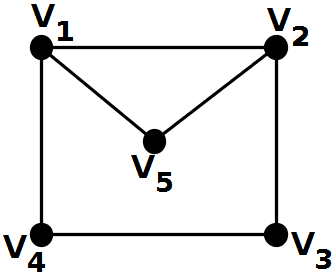
\includegraphics[width=3cm]{./img/envelope.png} & 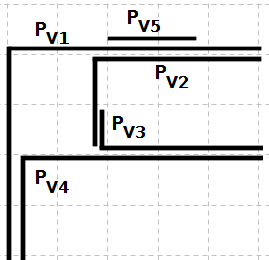
\includegraphics[width=4cm]{./img/envelopeHellyGradeTransparente.png} & 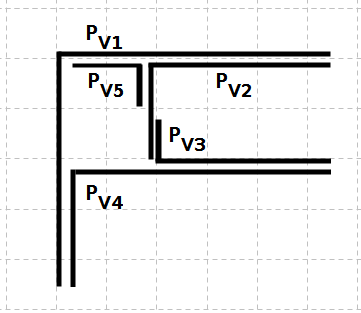
\includegraphics[width=4.6cm]{./img/envelopeNaoHellyGrade.png}
    \\
    \footnotesize \centering (a) Um grafo com  5 vértices & \footnotesize(b) Uma representação $B_1$-EPG que satisfaz a propriedade Helly & \footnotesize (c) Uma representação $B_1$-EPG que não satisfaz a propriedade Helly  \\

  \end{tabular}
\caption{Um grafo com 5 vértices em (a) e algumas representações de dobra simples: uma representação Helly em (b) e outra representação que não satisfaz a propriedade Helly em (c)} \label{fig:envelopeRepresentacoes}
\end{figure}



\subsection{O estudo de grafos EPG}

Um problema relacionado ao estudo de grafos EPG 
%Anterior ao estudo de grafos EPG existiu um problema similar, 
 é o problema de grafos de aresta-intersecção de caminhos em uma árvore, bem conhecido na literatura como EPT (Edge-intersection Graphs of Paths
in a Tree), ver~\cite{golumbic2004recognition}. Para grafos EPT, em particular, é resultado conhecido o valor dos parâmetros número de Helly, que  é 2, e do número de Helly forte, que é 3, resultados também em~\cite{golumbic2004recognition}. %A pesquisa de grafos EPG pode ser vista como uma extensão ao estudo pregresso de grafos EPT.

A respeito da complexidade do reconhecimento de grafos $B_k$-EPG, somente a complexidade de reconhecimento de três dessas subclasses de grafos foram determinadas: grafos
 $B_0$-EPG podem ser reconhecidos em tempo polinomial, uma vez que correspondem aos grafos de intervalo, ver~\cite{booth1976}. Em contraste, o reconhecimento de grafos $B_1$-EPG e $B_2$-EPG são problemas  $NP$-completos, ver~\cite{heldt2014, martin2017}, e o problema de reconhecimento de grafos $B_1$-EPG permanece $NP$-completo mesmo para caminhos $L$-shaped em grade, ver~\cite{cameron2016edge}.

Neste trabalho vamos estudar grafos que possuem uma representação EPG-Helly. Provamos que o problema de reconhecimento de grafos  $ B_1$-EPG-Helly é $NP$-completo. A propriedade Helly relacionada a representações de grafos EPG foi estudada por~\cite{golumbic2013} e~\cite{golumbic2009}. Em particular, eles determinaram o parâmetro  número de Helly forte de grafos $B_1$-EPG. 


 A pesquisa envolvendo grafos de aresta-intersecção de caminhos em grade é tópico relativamente novo na área de Teoria dos Grafos. As primeiras definições formais do problemas e aplicações foram apresentadas por Golumbic em 2009~\cite{golumbic2009}. Desde então diversas pesquisas têm sido conduzidas pela comunidade científica. Essas questões frequentemente abordam as representações dos caminhos, restrições quanto ao número de dobras em uma representação, entre outros. A seguir apresentaremos alguns trabalhos que conseguiram delimitar o \textit{número de dobras} para algumas classes de grafos.

No estudo de \citeauthor{alcon2016}, em~\cite{alcon2016}, os autores mostram que 3 dobras são suficientes para representar todos os grafos da classe de grafos arco-circular, i.e. eles estão em $B_3$-EPG. Adicionalmente, também mostram que existem grafos arco-circular que não podem ser representados com 2 dobras. Utilizando-se do fato de poder representar qualquer grafo arco-circular utilizando apenas um retângulo de uma grade de tamanho qualquer, o trabalho define a classe de grafos EPR e classificam os grafos arco-circular normais como sendo $B_2$-EPR, mostram ainda que existem grafos arco-circular normais que não são $B_1$-EPR. Finalmente, o trabalho dá uma caracterização de grafos $B_1$-EPR por uma família minimal de subgrafos induzidos proibidos e mostram que essa subfamília corresponde à uma subclasse de grafos normal arco-circular-Helly.

No trabalho de~\citeauthor{biedl2010}~\cite{biedl2010}, os autores mostram que 5 dobras são suficientes para representar todos os grafos planares e que 3 dobras são suficientes para representar todos os grafos outerplanar. Esses  resultados são posteriormente melhorados pelo trabalho de~\cite{daniel2014b}. Além desses resultados, o trabalho mostra que todo grafo planar bipartido possui representação EPG com 2 dobras e que todo grafo linha possui representação com 2 dobras. 


\citeauthor{daniel2014b} em~\cite{daniel2014b} mostraram que 4 dobras são suficientes para representar todos os grafos planares  e apresentam um algoritmo linear para encontrar essa representação com 4 dobras. Todavia, os autores ainda comentam que para alguns grafos planares, muitas vezes 3 dobras são suficientes para construção da representação. De fato, não é que simplesmente a maioria dos grafos planares poderiam ser construídos com 4 dobras, na verdade não se conhecem grafos planares que não podem ser desenhados utilizando apenas 3 dobras.   Isso deixa a seguinte questão: se 4 dobras são sempre suficientes para representar qualquer grafo planar então realmente são necessárias 4 dobras para representar qualquer grafo planar? Essa questão ainda está em aberto. Os autores ainda conjecturam que exista algum grafo onde para qualquer de suas representações EPG sempre existe pelo menos um caminho que precise utilizar as 4 dobras.

A Tabela~\ref{tab:limitesBenNumber} apresenta os principais limites conhecidos para o \textit{número de dobras}, notado como $b(G)$, de algumas classes de grafos.  


\begin{table}[h]
\caption{Algumas classes de grafos e limites conhecidos para o \textit{bend-number}}
\label{tab:limitesBenNumber}
\begin{center}
\begin{tabular}{|c|c|c|}
\hline 
Classe de Grafo & b(G) & Referência \\ 
\hline \hline  
Grafos de Intervalo & 0 & \cite{golumbic2009} \\ 
\hline 
Florestas & 1 & \cite{golumbic2009} \\ 
\hline 
Outerplanar & 2 & \cite{daniel2014b} \\ 
% \hline 
% Planar & 5 e dim $(n-1)\times(2n-3)$ & \cite{biedl2010} 2010\\ 
\hline 
Planar & $3 \leq - \leq 4$ & \cite{daniel2014b}\\ 
\hline  
Bipartido Planar & 2 & \cite{biedl2010} \\ 
\hline 
Grafo Linha & 2 & \cite{biedl2010} \\ 
\hline 
dgn(G)~\footnote{Degeneracy - uma orientação acíclica de $G$ que é $k-$regular } $\leq k$ & $2k-1$ & \cite{daniel2014b} \\ 
\hline 
tw(G)~\footnote{Treewidth} $\leq k$ & $2k-2$ & \cite{daniel2014b} \\ 
\hline 
Degree $\leq \Delta$ & $ 	\lceil \frac{\Delta}{2}\rceil\leq - \leq\Delta $ & \cite{daniel2014b} \\ 
\hline 
Arco-circular & 3 & \cite{alcon2016} \\ 
\hline 
\end{tabular} 
\end{center}
\end{table}

Além dos resultados citados para limites do número de dobras de algumas classes de grafos, existem muitos trabalhos que caracterizam outros tipos de grafos não citados nessa tabela, como o trabalho de~\citeauthor{ries2009}~\citep{ries2009} que caracteriza os grafos cordais, livres de garra, touro e diamante que possuem uma representação $B_{1}-$EPG. Nesse mesmo artigo há também uma caracterização de alguns grafos split, com restrição ao tamanho do conjunto independente ou da clique, por subgrafos proibidos. O trabalho ainda tem um resultado interessante que mostra que a vizinhança de todo vértice de um grafo $B_1$-EPG induz um grafo fracamente cordal.

Apesar de ser possível encontrar várias pesquisas em grafos EPG investigando o número de dobras, os interesses de estudos nessa classe de grafos se estendem a outros problemas clássicos, os quais podemos citar a seguir.

Em~\citet{cohen2014} é apresentado um algoritmo de reconhecimento de tempo linear para cografos $B_{1}-$EPG por uma família de subgrafos induzidos proibidos. O algoritmo que o trabalho apresenta utiliza a co-árvore do cografo no processo de reconhecimento.
 
 Algoritmos aproximativos para coloração de grafos $B_1$-EPG foram estudados em~\cite{epstein2013approximation}. O trabalho citado mostra que o problema de coloração e o problema de conjunto independente máximo são ambos $NP$-completos para grafos $B_1$-EPG mesmo quando a representação EPG é dada. Os autores apresentam um algoritmo  4-aproximativo que resolve ambos os problemas, assumindo que a representação EPG é dada. O trabalho ainda mostra que a clique máxima pode ser encontrada de forma eficiente em grafos $B_1$-EPG mesmo quando a representação não é dada.
 
 Problemas de clique-coloração em grafos $B_1$-EPG foram estudados por~\cite{bonomo2017clique}. Os autores consideram o problema de clique coloração e mostram que grafos $B_1$-EPG são 4-clique-coloríveis e apresentam um algoritmo de tempo linear para resolver o problema.

Além dos trabalhos citados podemos mencionar também como pesquisa frequente com relação aos grafos EPG o estudo de complexidade \cite{daniel2014b, martin2017}, área da grade necessária para representação de um grafo cujo grau máximo é $\Delta(G)$ \cite{Asinowski2009}, e muitos outros.

Dentre os diversos temas estudados é possível perceber que a pesquisa que relaciona grafos EPG cujas representações satisfazem a propriedade Helly é escassa.
A dificuldade de reconhecimento de pouquíssimas classes de grafos EPG é conhecida, e ainda para valores de $k$ pequenos somente.  %Dessa forma, diante das aplicações apresentadas e dos trabalhos levantados na revisão da literatura, é possível perceber que pelo menos uma das propostas deste trabalho, que é investigar a dificuldade de reconhecimento de grafos $B_1$-EPG-Helly, é viável e factível do ponto de vista prático. Logo, 
 No capítulo seguinte nos dedicaremos a expor os principais resultados obtidos até aqui.

%\cite{Asinowski2009} mostrou que não existe um k para o qual todo grafo é B_k-EPG, somente uma quantidade exponencial de grafos pertencem a B_k-EPG para algum k dado.